\documentclass[a4paper,12pt]{article}
\usepackage{latexsym}
\usepackage{graphicx}
\usepackage{epsfig}
\usepackage{float}
\usepackage{natbib}
\usepackage{listings}
\usepackage{amsmath}
\graphicspath{{./}}
\DeclareGraphicsExtensions{.jpg}
\author{Howard Kinsman}
\title{Cosmology Tutorial 8}
\begin{document}
\maketitle
\section{}
\subsection{}
\begin{flalign*}
& \rho=\left(\frac{R}{R_0}\right)^{-3} 5\times10^{-28} &\\
& \frac{R}{R_0}=(1+z)^{-1}=8\times10^{-4} &\\
& \rho=1.7\times10^9\times5\times10^{-28}\approx8.6\times10^{-19}kg m^{-3} &\\
& T=2.7(1+z)\approx 3000K
\end{flalign*}
\subsection{}
\begin{flalign*}
& 3.6\times10^9\times3000^{\frac{3}{2}}\left(8.6\times10^{-19}\right)^{\frac{-1}{2}} &\\
& M_J\approx6\times10^5 M_\odot 
\end{flalign*}
Globular clusters and possibly giant molecular clouds have around this mass.
\newline
Fractional fluctuations from statistics are very small $(3\times10^{-32})$. Fluctuations grow proportional to the scale factor so from $z=100$ to $z=10$ they would only grow by
a factor of 10. This therefore implies that there should have been a 'seed' perturbation as part of initial conditions of big bang e.g. dark matter (WIMPS).
\section{}
\subsection{}
In radiation era fluctuations don't grow because of damping due to photons random walking out of high pressure regions.
\newline
The problem is alleviated if WIMPS are involved because dark matter decouples earlier than baryonic matter and so can start to collapse earlier as it feels no pressure.
\subsection{}
\begin{figure}[H]
\centering
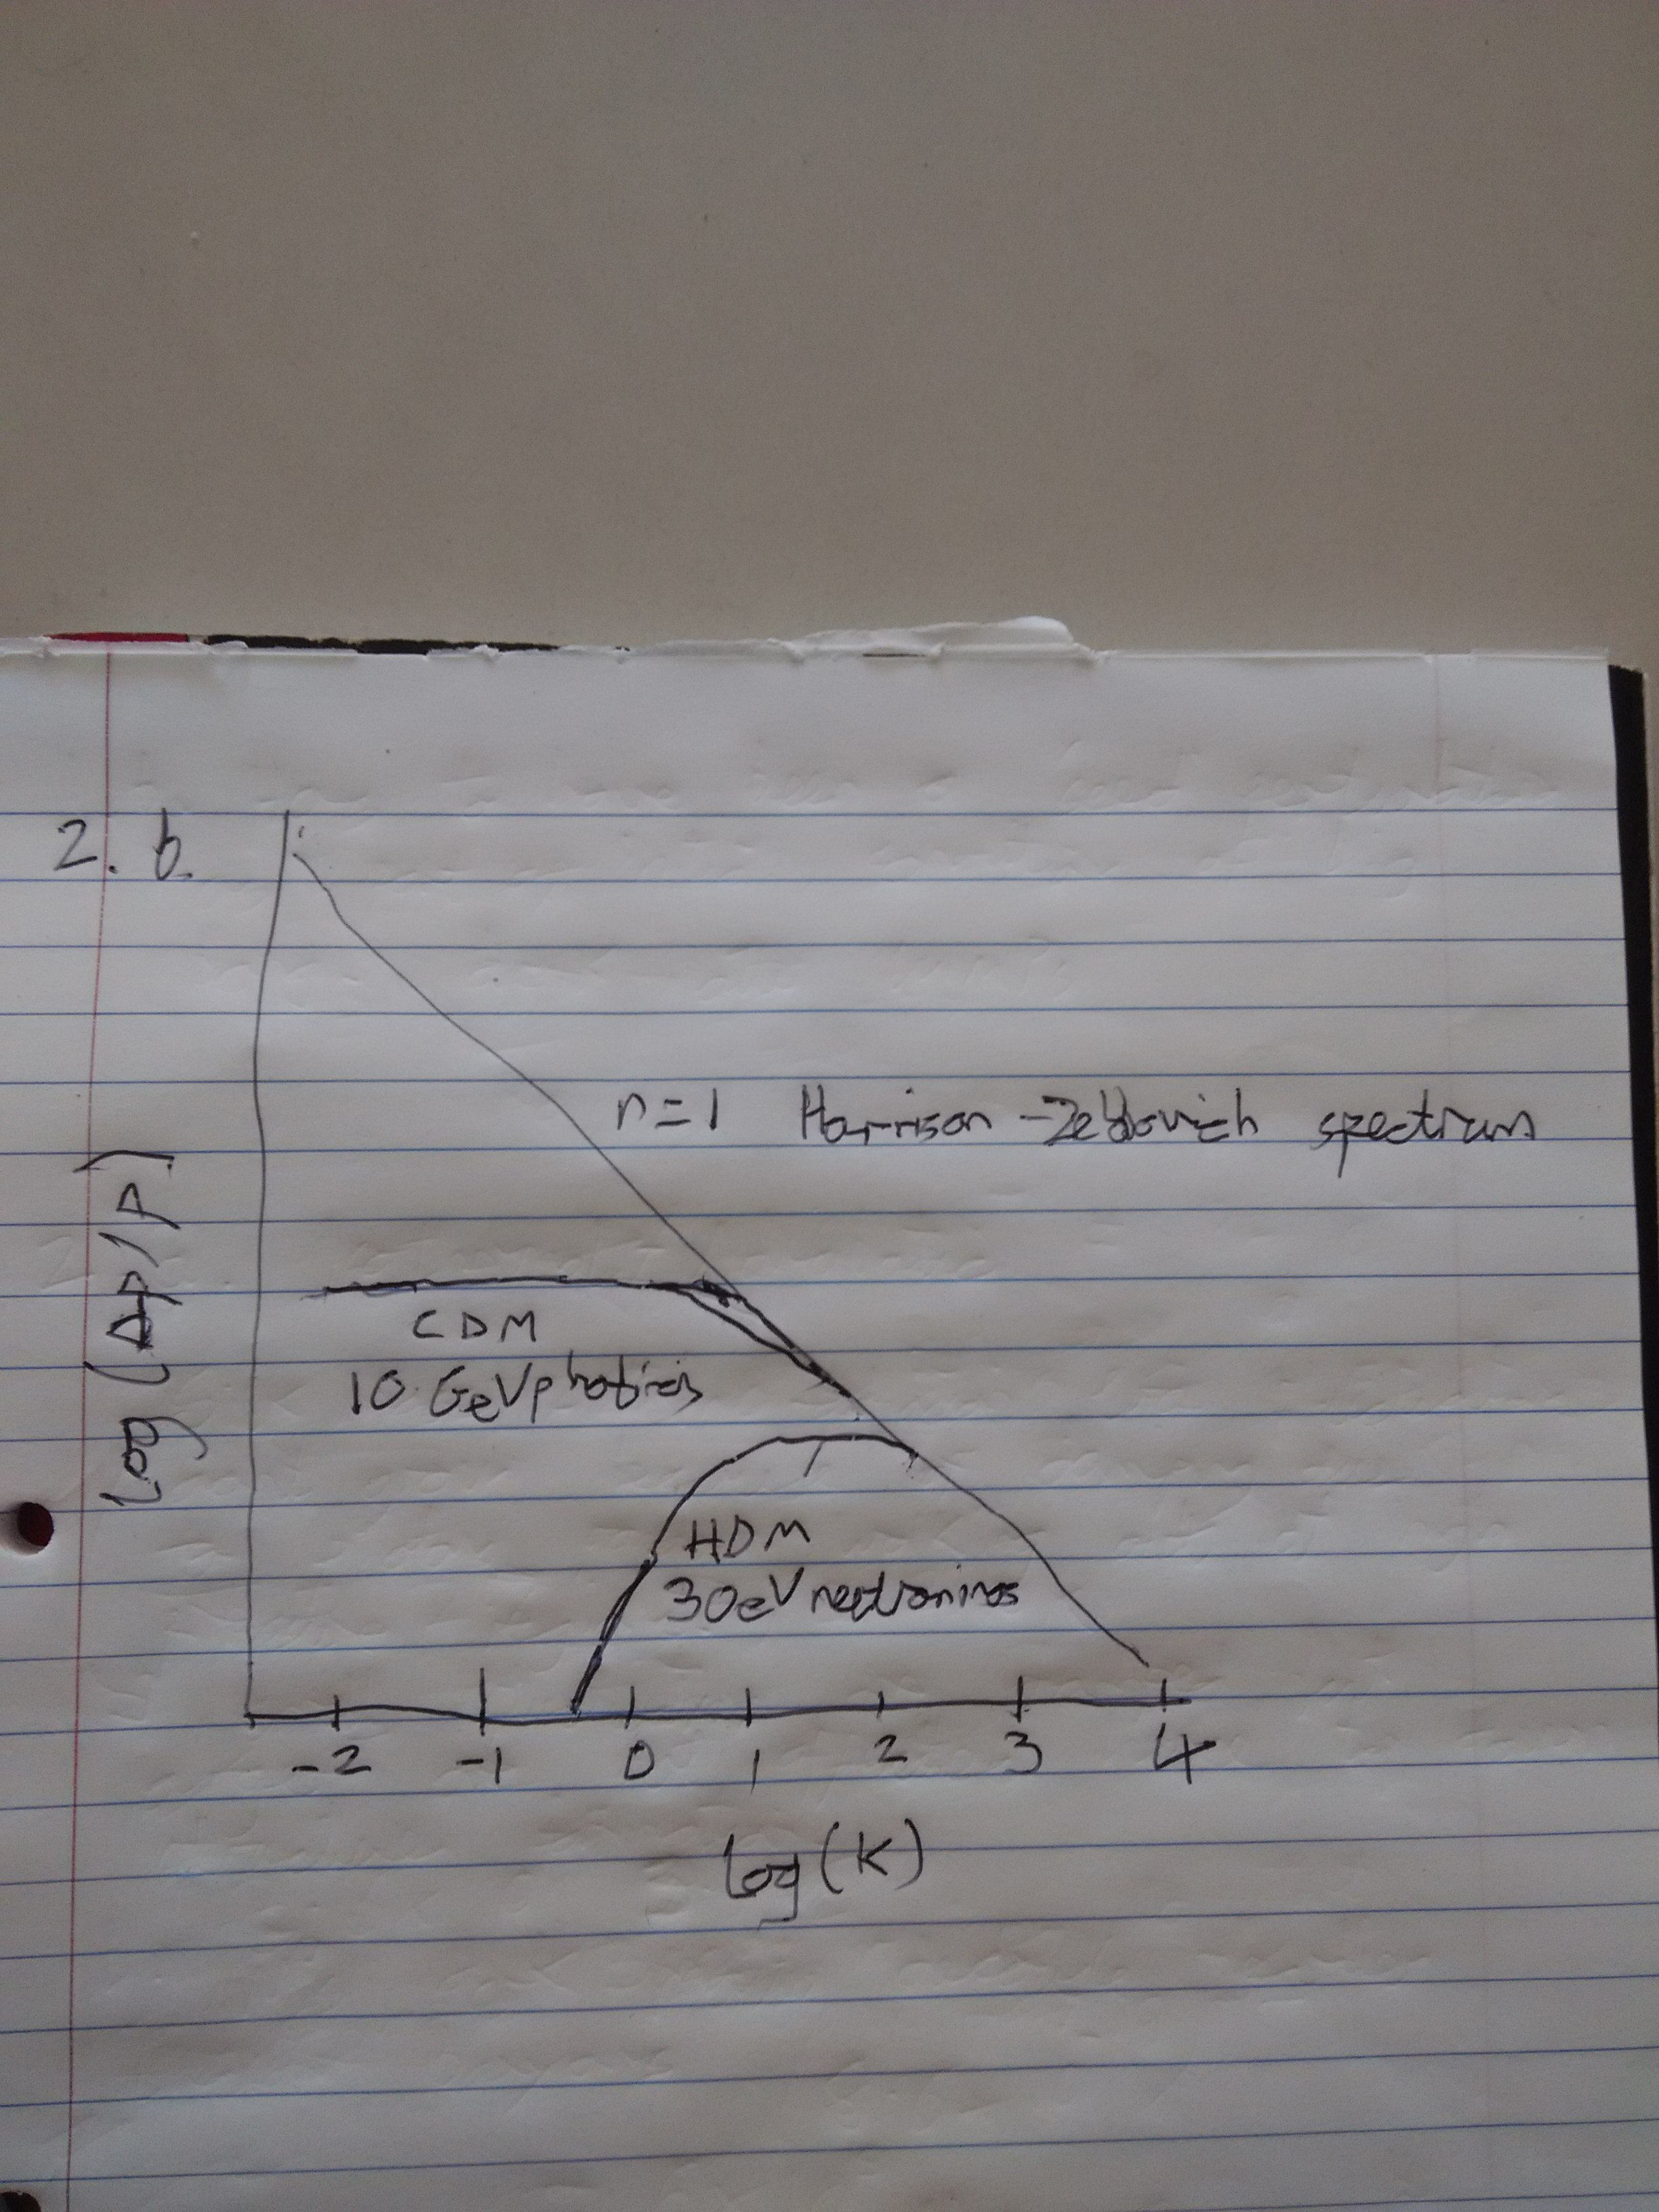
\includegraphics[width=.9\textwidth]{./pic.jpg}
\caption{}
\label{fig:1}
\end{figure}
\subsection{}
With CDM these particles decouple early and are non-relativistic earlier. Fluctuations are damped at all scales and so as small things collapse first
this leads to bottom up structure formation.
With HDM these particles are relativistic until recombination. They become damped due to free-streaming. Fluctuations are wiped out up to a large mass
which leads to top down structure formation.
\section{}
\subsection{}
\begin{flalign*}
& \dot{R}^2=\frac{8\pi G}{3}\rho_{r,0}\frac{R_0^4}{R^2}-kc^2 &\\
& kc^2=R_0^2 H_0^2(\Omega_0-1) &\\
& \dot{R}^2=\frac{8\pi G}{3}\rho_{r,0}\frac{R_0^4}{R^2}-R_0^2 H_0^2(\Omega_{0,r}-1) &\\
& \left(\frac{\dot{R}}{R}\right)^2=H^2=\frac{8\pi G}{3}\rho_{r,0}\frac{R_0^4}{R^4}-\frac{R_0^2}{R^2} H_0^2(\Omega_{0,r}-1) &\\
& =\frac{8\pi G}{3}\rho_{r,0}(1+z)^4-(1-z)^2 H_0^2(\Omega_{0,r}-1) &\\
& =\Omega_{0,r}H_0^2(1+z)^4-(1+z)^2H_0^2(\Omega_{0,r}-1) &\\
& =H_0^2(1+z)^2\left[\Omega_{0,r}z^2+2\Omega_{0,r}z+\Omega_{0,r}-\Omega_{0,r}+1\right] &\\
& =H_0^2(1+z)^2\left[\Omega_{0,r}z^2+2\Omega_{0,r}z+1\right] &\\
& =H_0^2(1+z)^2\left[1+\Omega_{0,r}(2z+z^2)\right] 
\end{flalign*}
\subsection{}
\begin{flalign*}
& \Omega=\frac{8\pi G}{3H^2} &\\
& \rho=\rho_0(1+z)^4 &\\
& \Omega(z)=\frac{8\pi G\rho_0(1+z)^4}{3H_0^2(1+z)^2\left[1+\Omega_{0,r}(2z+z^2)\right]} &\\
& =\frac{8\pi G\rho+0(1+z)^2}{3H_0^2\left[1+\Omega_{0,r}(2z+z^2)\right]} &\\
& =\frac{\Omega_{0,r}(1+z)^2}{1+\Omega_{0,r}(2z+z^2)}
\end{flalign*}
That is as far as I got.
%\begin{thebibliography}{1}
%\end{thebibliography}
\end{document} 